%%%%% Physik Kompendium Nr.2 %%%%%
%% 06 -- Der Siebkreis %%

Schwingkreise sind Schaltkreise, die aus den zwei Wechselstromwiderständen Spule und Kondensator sowie (in der Theorie) aus einem Ohm'schen Widerstand bestehen. Daher nennt man sie auch LC- oder LCR-Schaltungen. In der Praxis könnte auf einen Ohm'schen Widerstand verzichtet werden, da eine reelle Spule immer auch einen Ohm'schen Widerstand besitzt, denn sie besteht aus Draht. 

Diese Stromkreise haben in der Wechselstromumgebung frequenzabhängige Eigenschaften (Siehe \referenz{subsec:Frequenzabhaengigkeit}), sowie eine Resonanzfrequenz, bei der sich die Größe der beiden Wechselstromwiderstände die Waage halten und der Blindwiderstand folglich $0$ ist (Siehe \gleichungsreferenz{eq:BlindwiderstandSumme}).

\subsection{Natürliche Schwingkreis}

Der Schwingkreis\footnote{„SchwingkreisSchaltung“ von Till Blaha - Eigenes Werk. Lizenziert unter Gemeinfrei} ist ein essentieller Bestandteil von Oszillatoren, also Schwingungsgeneratoren. 

\begin{figure}[h!]
	\centering
	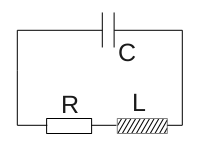
\includegraphics[width=0.5\textwidth]{Schwingkreis}
	\caption{Diagramm des Schwingkreises}
\end{figure}

Im Stromkreis sind alle Bauteile in Reihe geschaltet und es gibt keine externe Spannungsquelle. Jedoch ist der Kondensator zu Anfang geladen; er trägt anfangs die gesamte Energie des Aufbaus.

\begin{figure}[h!]
	\centering
	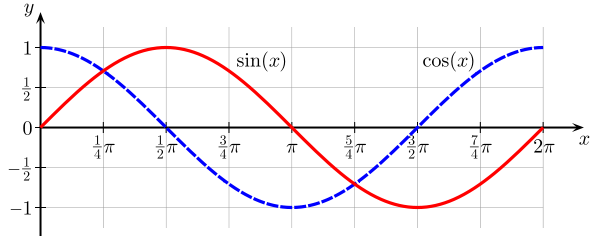
\includegraphics[width=0.8\textwidth]{SchwingkreisGraph}
	\caption{Spannung (blau) und Stromstärke (rot) in einem Schwingkreis über der Zeit}
\end{figure}

Sobald der Kreis, bspw. über einen Schalter, geschlossen wurde, entlädt sich der Kondensator; die Spannung fällt. Durch die Selbstinduktion an der Spule steigt die Stromstärke jedoch langsam an, welche ohne diesen induktiven Widerstand sofort nach dem schließen des Schalters auf ihrem Maximum gewesen wäre.

Auch wenn der Kondensator vollständig entladen ist (Stelle $\frac{1}{2}\pi$ im Diagramm\footnote{„Sine cosine one period“ von Geek3 - Eigenes Werk. Lizenziert unter CC BY 3.0 über Wikimedia Commons - \url{https://commons.wikimedia.org/wiki/File:Sine_cosine_one_period.svg}}), also die Spannung $0V$ beträgt, ist immer noch eine Stromstärke messbar, da der Ladungsfluss durch die Selbstinduktion in der Spule verzögert ist. Allerdings ist der Verlauf der Stromstärke fallend, da keine weitere Ladung mehr in die Spule fließt (der Kondensator ist entladen). An der Stelle $\frac{1}{2}\pi$ trägt der Kondensator keine Ladung und die maximale Stromstärke ist erreicht, was bedeutet, dass zu diesem Zeitpunkt die gesamte Energie der Schaltung im Magnetfeld der Spule gespeichert ist.

Im Abschnitt zwischen $\frac{1}{2}\pi$ und $\pi$ ist die Spannung negativ, das heißt die Kondensatorplatten wurden und werden mit anderer Polung als am Anfang des Versuches geladen. Trotzdem fließen immer noch weitere Ladungen auf die Kondensatorplatten, da der Stromfluss durch die Spule verzögert wurde. Sobald der Kondensator vollständig geladen wurde ($\pi$), fließt kein Strom mehr (Stromstärke ist $0A$), das heißt, es gibt kein Magnetfeld mehr und die gesamte Energie ist, wie zu Beginn, im Kondensator gespeichert.

Dieser Vorgang wiederholt sich periodisch, bis die Ladungen durch den Verbraucher (in diesem Fall den Ohm'schen Widerstand) verbraucht wurden, in diesem Fall in Wärme umgewandelt wurden.

\subsubsection{Resonanzfrequenz}

Die Resonanzfrequenz ist die Frequenz, bei der die Impedanz so klein wie möglich ist, das heißt, die angestrebte Frequenz, die oszilliert wird.

Um eine kleinstmögliche Impedanz zu erreichen, muss der Blindwiderstand $0$ sein, woraus folgt, der reelle Teil des Gesamtwiderstands (der Ohm'sche Widerstand) die gesamte Impedanz ausmacht. Aus Gleichung \ref{eq:BlindwiderstandSumme} abgeleitet, gilt:

\begin{align}	\label{eq:ResonanzfrequenzSchwingkreis}
\begin{split}
	X_L - X_C &= 0 \\
	X_L &= X_C \\
	\omega \cdot L &= \frac{1}{\omega \cdot C} \\
	\omega ^2 &= \frac{1}{C \cdot L} \\
	\omega &= \frac{1}{\sqrt{C L}} \\	
	f &= \frac{1}{2 \pi \cdot \sqrt{C L}} \\
\end{split}
\end{align}


\subsection{Siebkreis}

Der Siebkreis (manchmal auch LCR-Schaltung oder Reihenschwingkreis genannt) ist eine bekannte technische Anwendung, deren Aufgabe es ist, aus einem bestehenden Signal (angedeutet im Diagramm\footnote{„SiebkreisSchaltung“ von Till Blaha - Eigenes Werk. Lizenziert unter Gemeinfrei}) einen bestimmten Frequenzbereich \glqq herauszufiltern\grqq , will sagen, dort die geringste Impedanz und folglich die höchste Stromstärke aufzuweisen.

\begin{figure}[h!]
	\centering
	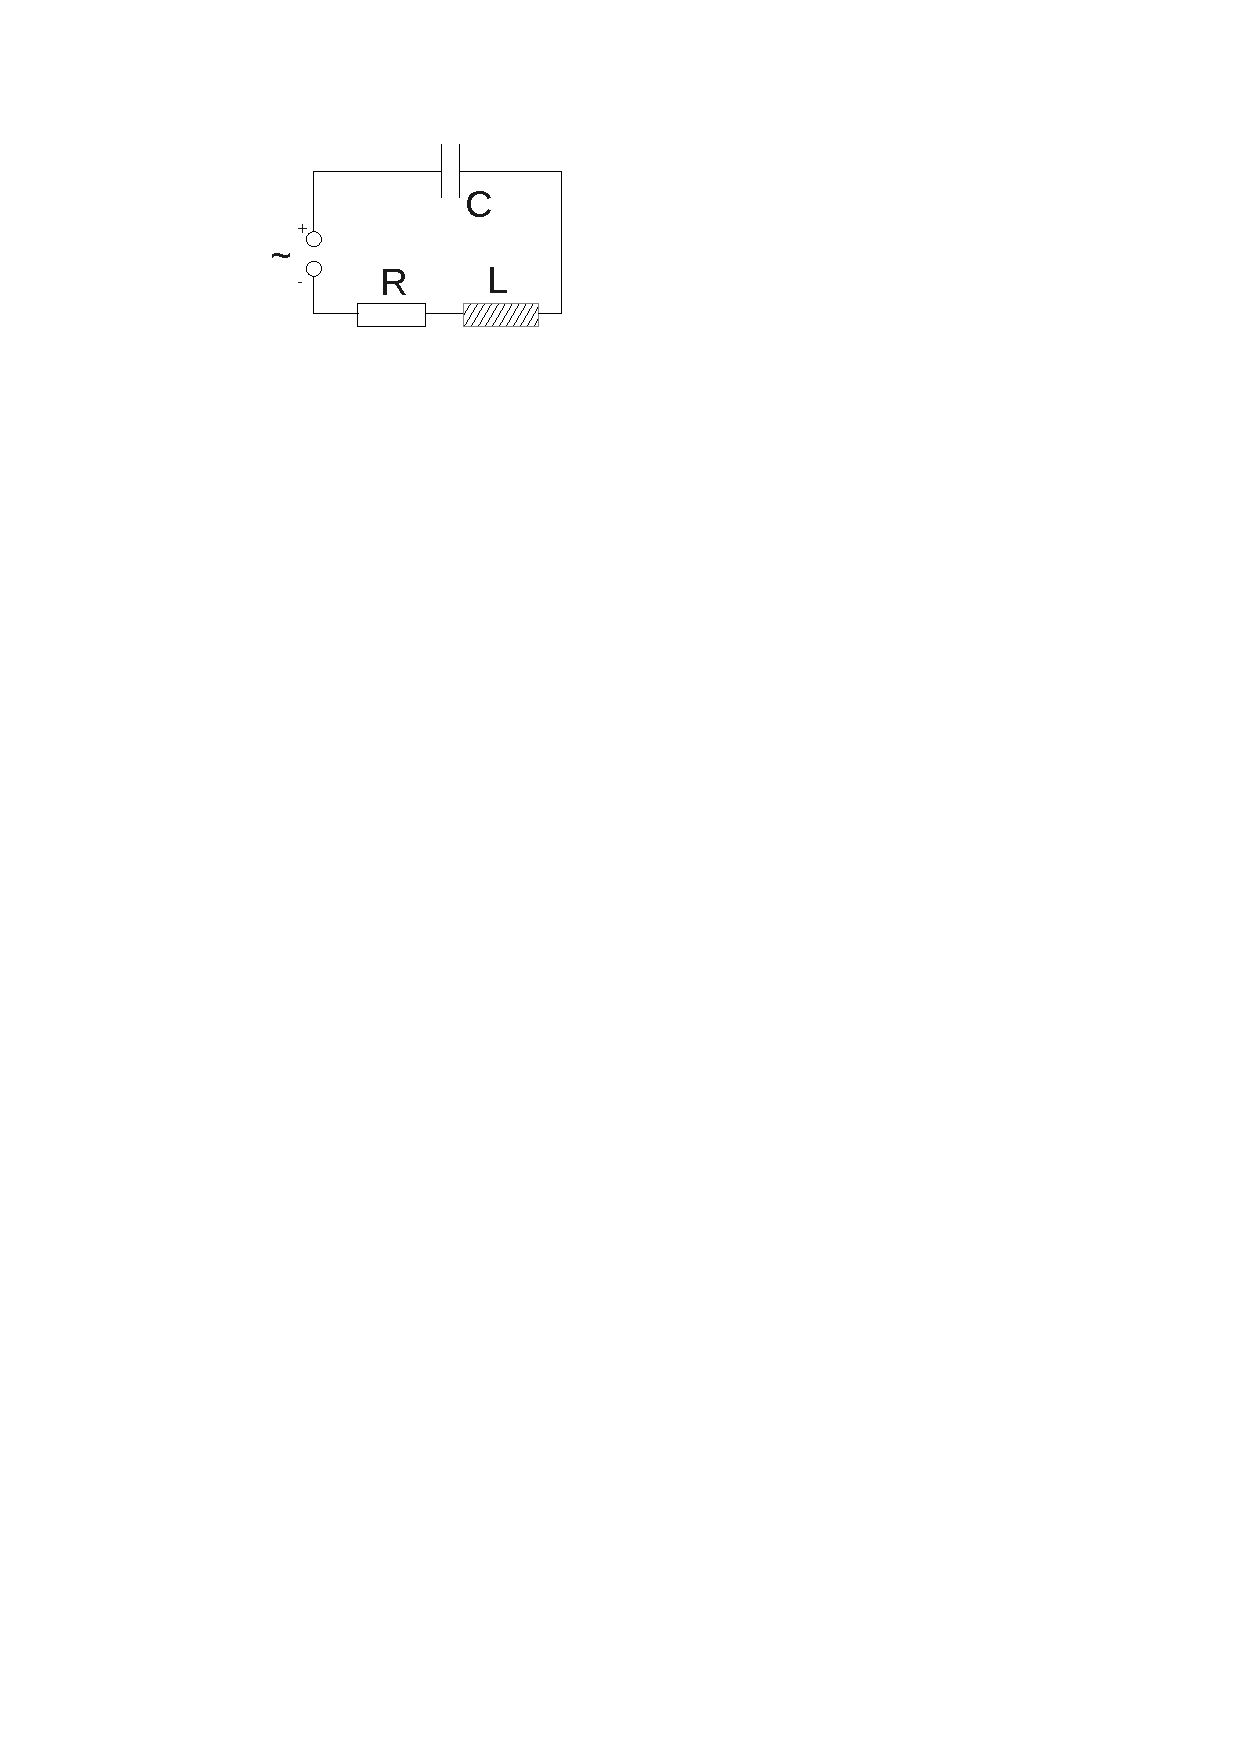
\includegraphics[width=0.5\textwidth]{Siebkreis}
	\caption{Diagramm eines Siebkreises}
\end{figure}

Der Kondensator \glqq schneidet\grqq{} die hohen Frequenzen \glqq ab\grqq , die Spule die tiefen. Siehe Sektionen \referenz{subsec:Frequenzabhaengigkeit} und \referenz{subsec:AuswirkungenWiderstand} für weitere Erläuterungen.

Der Frequenzbereich, also dessen Lage im Spektrum und dessen Breite, wird durch die Daten der Bauteile bestimmt.


\subsubsection{Resonanzfrequenz}

Die Resonanzfrequenz, also die Frequenz mit dem geringsten Gesamtwiderstand, lässt sich genauso berechnen wie beim Schwingkreis:

\begin{align}	\label{eq:ResonanzfrequenzSiebkreis}
\begin{split}
	X_L - X_C &= 0 \\
	f &= \frac{1}{2 \pi \cdot \sqrt{C \cdot L}}
\end{split}
\end{align}

Ist die Frequenz des Wechselstroms nun höher als die Resonanzfrequenz ist die Impedanz höher, da der induktive Widerstand größer wird; bei niedrigerer Frequenz nimmt der kapazitive Widerstand zu. Dieses Diagramm\footnote{„SiebkreisGraph“ von Till Blaha - Eigenes Werk. Lizenziert unter Gemeinfrei} zeigt eine mögliche Stromstärke/Widerstand-über-Frequenz-Kurve:

\begin{figure}[h!]
	\centering
	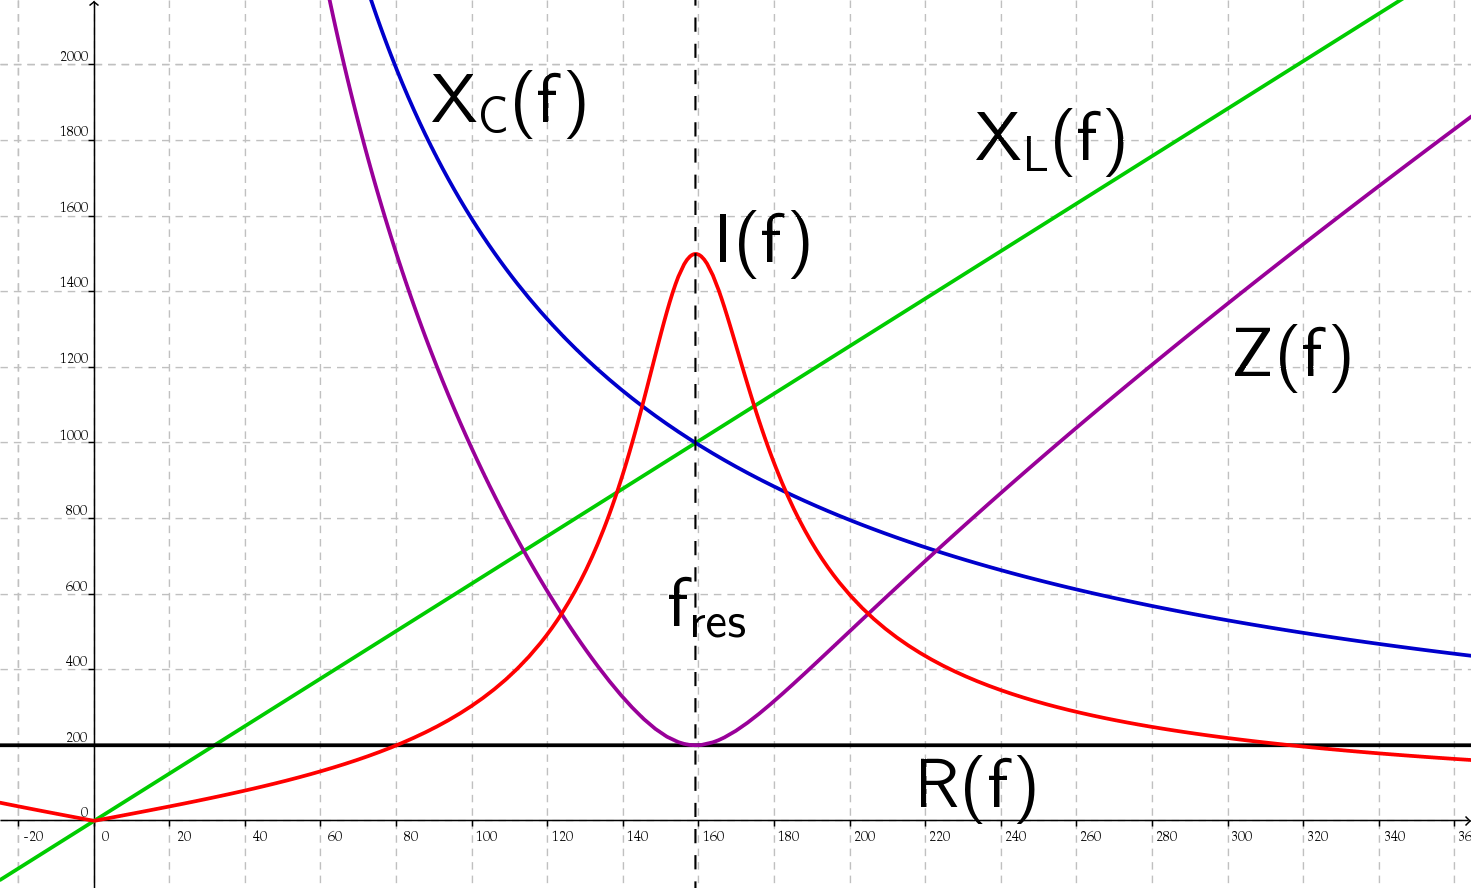
\includegraphics[width=\textwidth]{SiebkreisGraph}
	\caption{Die 3 Widerstände, Impedanz und Stromstärke mit fiktiver y-Skalierung. Frequenz auf der x-Achse. Man beachte die Schnittstelle von $X_L$ und $X_C$ die Gleichzeitig der Tiefpunkt der Impedanz $Z$ und damit der Hochpunkt der Stromstärke $I$ ist.}
\end{figure}




